\chapter{Estado del arte}

\vspace{-0.5cm}

\begin{flushright}
  \emph{\guillemotleft Cita o lo que quieras\guillemotright}\\ \textbf{Author}
\end{flushright}
\hyphenation{}
\grayMinitoc

\parindent=16mm

\CAPstart{E}{n}~el siguiente capítulo de este TFM se presentarán los conceptos y herramientas que es necesario comprender para poder seguir correctamente el flujo de este trabajo.

\section{Iteraciones}

\subsection{Iteración 1 - Modelo del sistema}
\label{res:iteracion1}
Esta iteración se centra en la descripción del problema planteado y en la elección de las herramientas a utilizar para el desarrollo de un diseño \textit{hardware} capaz de cumplir con los requisitos expuestos en \ref{sec:requisitos}. En este punto, se ha analizado en detalle el conjunto de dichos requisitos, además de realizar diversas preguntas, para entender mejor la problemática.

Con el objetivo de cumplir dichos requisitos, se pretende desarrollar un diseño \textit{hardware} capaz de realizar una operación concreta, siendo, en el contexto de este trabajo, el reverso de bits de un número entero de 32 bits. Para ello, se ha optado por un esquema basado en colas \ac{FIFO}, de las cuales ya se detalló tanto su concepto como sus ventajas en \ref{st:colasFifo}. La idea es, por tanto, hacer sencillo el paso de datos al acelerador, así como la recepción de los resultados. Las colas FIFO, al tener memoria interna, proporcionan un mecanismo sencillo y relativamente seguro de transmisión.

Para realizar este diseño, es necesario realizarlo en base a una metodología. En el contexto de este trabajo, se ha optado por alinear el esfuerzo a las metodologías basadas en herramientas EDA, ello implicando el uso de programas software que estén adecuados al flujo de este tipo de metodologías. Por ello, se ha optado por seleccionar Vitis HLS y Vivado como programas para el diseño de este hardware. Ambas son herramientas de la misma compañía, Xilinx, lo que repercute en, teóricamente, una mejor integración entre ellas, lo que agiliza el desarrollo. Además, han sido presentadas en el máster, lo que las hace más fáciles de utilizar que herramientas de la competencia, como las de la empresa Cadence. Para pruebas, ya con un SoC simulado, se ha optado por el uso de X-HEEP, que permite la creación de núcleos RISC-V de múltiples tipos, así como simulaciones a nivel \textit{hardware} gracias a Verilator, y con soporte para FreeRTOS, lo que proporciona flexibilidad a la hora de realizar cualquier tipo de despliegue.

Por tanto, a modo de resumen, el resultado de esta iteración ha sido:

\begin{enumerate}
    \item Se han analizado los requisitos
    \item Se ha proporcionado un marco de trabajo para el desarrollo técnico del proyecto
    \item Se ha dado respuesta a cómo comunicarse a la entrada y a la salida del módulo acelerador
    \item Se han seleccionado e instalado las herramientas a utilizar tras valorar diversas opciones
\end{enumerate}

\subsection{Iteración 2 - Desarrollo del diseño hardware}

En esta fase se ha realizado el esquema correspondiente al un diseño hardware que sea capaz de satisfacer los requisitos y cumplir con el problema planteado. Si bien se estudiaron varios mecanismos, tal y como se expone en \ref{res:iteracion1}, se ha optado finalmente por un esquema basado en colas FIFO. 

\subsubsection{Diseño original}
Para lograr el diseño final, han sido necesario un refinamiento del planteamiento inicial. Originalmente, se ideó un esquema de 5 módulos, imposible de mostrar, debido a que los archivos del proyecto fueron sobreescritos durante la optimización del mismo. Estos módulos son los siguientes:

\begin{enumerate}
    \item \textbf{Cola FIFO de entrada}: cuyo objetivo es guardar datos para, llegados a un \textit{threshold}, comenzar a mandarlos al siguiente. Mediante una señal de escritura, se escriben los datos. A partir de entonces, es posible leerlos por la salida.

    \item \textbf{Cola FIFO de conversión a AXI-Stream}: este módulo se comunica con el acelerador con señales AXI-Stream de entrada. Recibe los datos guardados por el módulo anterior, y, recibidos todos (ese \textit{threshold}) el módulo activa las señales AXI-Stream para mandar los datos al módulo acelerador

    \item \textbf{Acelerador generado con Vitis HLS}: este módulo se basa en el protocolo AXI-Stream, de forma que, al activarse las señales de su entrada, comienza a recibir los datos y a procesarlos uno a uno hacia el siguiente módulo y activa señales de salida.

    \item \textbf{Cola FIFO de conversión AXI al formato de origen}: este módulo se comunica con el acelerador con señales AXI-Stream de salida. Recibe los resultados y, al activarse sus entradas AXI-Stream, comienza a mandarlos al siguiente.

    \item \textbf{Cola FIFO de salida}: este módulo obtiene los datos resultado del módulo conversos de AXI-Stream a datos puros. Una vez recibidos todos, los devuelve por su salida de datos.
\end{enumerate}

Este esquema no ha sido el definitivo, por varias razones:

\begin{itemize}
    \item \textbf{Demasiados componentes para la tarea a realizar}: se puede agruparlos sin aumentar en exceso la lógica de control del diseño global
    \item \textbf{Inicialización del acelerador inconsistente}: no se tiene lógica alguna para activar el módulo HLS, activándose ésta al inicio, siendo necesario un tiempo extra para un correcto funcionamiento
    \item \textbf{Falta de señales de control}: solo se devuelven los datos del acelerador, sin tener señales de intermedias que indiquen el estado de la ejecución
\end{itemize}

\subsubsection{Diseño final}
\begin{adjustwidth}{1.5cm}{}
\textbf{Descripción} \vspace{0.25cm} \\
Finalmente, se ha optimizado el diseño original, el cual se presenta en \ref{fig:disenoFinal}, añadiendo señalizaciones de control y estado, y reduciendo a tres el número de módulos, que son:

\begin{enumerate}
    \item \textbf{Cola FIFO de conversión a AXI-Stream}: este módulo se comunica con el acelerador con señales AXI-Stream de entrada. Una vez que la señal de \emph{reset} deja de estar activa, se activa la señal de control \emph{start\_accel} que activa el módulo acelerador, el cual requiere de una cantidad reducida de ciclos para inicializarse. Los datos fluyen de la siguiente forma: al activarse la señal de control \emph{start}, se comienza a guardar datos en \textit{buffer}. Llegados al \textit{threshold} de 4 valores, el módulo activa las señales AXI-Stream y manda los datos al módulo acelerador.
    \item \textbf{Acelerador generado con Vitis HLS}: este módulo emplea en el protocolo AXI-Stream para comunicarse; ya inicializado gracias a \emph{start\_accel}, al activarse las señales de su entrada y a recibir datos, comienza a procesarlos uno a uno y los manda hacia el siguiente módulo activando sus señales AXI-Stream de salida.
    \item \textbf{Cola FIFO de conversión AXI al formato de origen}: este módulo se comunica con el acelerador con señales AXI-Stream de salida. Recibe los resultados y, al activarse sus entradas AXI-Stream, comienza a devolverlos por su salida, a la vez que activa la señal de estado \emph{done}.
\end{enumerate}

\begin{figure}[!ht]
    \centering
    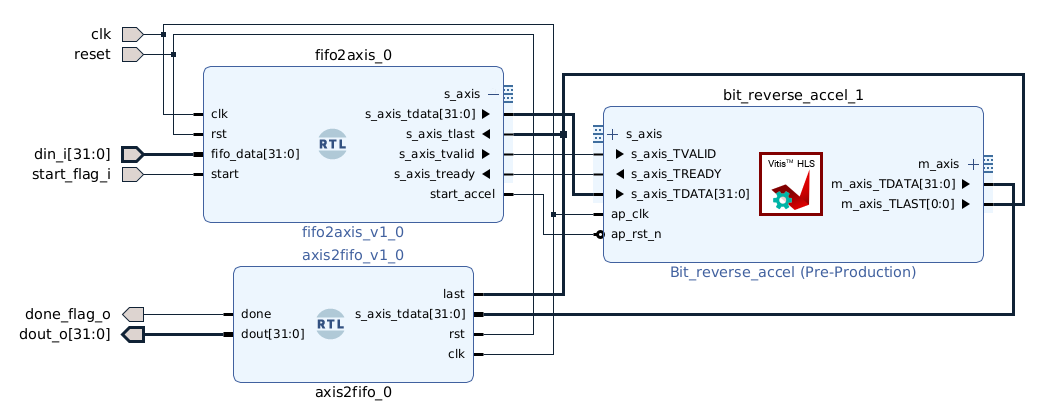
\includegraphics[width=12cm]{figures/disenoFinal.png}
    \caption{Digrama de bloques final}
    \label{fig:disenoFinal}
\end{figure}
\end{adjustwidth}

\vspace{0.4em} % Espacio vertical entre párrafos

\begin{adjustwidth}{1.5cm}{}
\textbf{Señales principales del diseño} \vspace{0.25cm} \\
En esta sección se presentan en \ref{tbl:senalesDiseno} las señales más importantes del diseño hardware realizado en este trabajo. 

\begin{table}[H]
\centering
\resizebox{10cm}{!} {
    \begin{tabular}{|c|c|}
    \hline
    \textbf{Señal} & \textbf{Descripción} \\
    \hline
    clk & Señal de reloj principal del sistema. \\
    \hline
    reset / rst & Señal de reset (activa en alto), reinicia los módulos. \\
    \hline
    din\_i[31:0] & Entrada de datos de 32 bits hacia el sistema. \\
    \hline
    start\_flag\_i & Señal de inicio para habilitar el envío de datos. \\
    \hline
    fifo\_data[31:0] & Datos provenientes del FIFO hacia el bus AXI-Stream. \\
    \hline
    s\_axis\_tdata[31:0] & Bus de datos de entrada (AXI-Stream). \\
    \hline
    s\_axis\_tvalid & Indica que los datos en \texttt{s\_axis\_tdata} son válidos. \\
    \hline
    s\_axis\_tready & Señal de "ready" del esclavo, indica que puede aceptar datos. \\
    \hline
    s\_axis\_tlast & Indica la última transferencia de un paquete AXI-Stream. \\
    \hline
    m\_axis\_tdata[31:0] & Bus de datos de salida (AXI-Stream). \\
    \hline
    m\_axis\_tlast & Señal de fin de paquete de datos en la salida. \\
    \hline
    done\_flag\_o & Señal que indica finalización del procesamiento. \\
    \hline
    dout\_o[31:0] & Datos de salida del sistema (32 bits). \\
    \hline
    ap\_clk & Reloj para el acelerador HLS. \\
    \hline
    ap\_rst\_n & Reset del acelerador HLS (activo en bajo). \\
    \hline
    \end{tabular}
}
\label{tbl:senalesDiseno}
\caption{Principales señales del diseño}
\end{table}

Con estas señales, el sistema comienza recibiendo los datos de entrada a través de la señal \emph{din\_i[31:0]}, los cuales son almacenados temporalmente en un FIFO. 
Cuando la señal \emph{start\_flag\_i} habilita el proceso, el bloque \emph{fifo2axis} toma los datos del FIFO y los coloca en la interfaz AXI-Stream, 
usando \emph{s\_axis\_tdata} junto con las señales de control \emph{s\_axis\_tvalid}, \emph{s\_axis\_tready} y \emph{s\_axis\_tlast} para garantizar la correcta transmisión. 
Estos datos entran al acelerador \emph{bit\_reverse\_accel}, implementado en HLS, donde se realiza el procesamiento de inversión de bits. 
Una vez procesados, los resultados son enviados a través de la interfaz de salida AXI-Stream (\emph{m\_axis\_tdata} y \emph{m\_axis\_tlast}) hacia el bloque \emph{axis2fifo}, 
que convierte nuevamente la transmisión en datos almacenados en FIFO. 
Finalmente, los resultados procesados se entregan en la salida \emph{dout\_o[31:0]}, mientras que la señal \emph{done\_flag\_o} indica la finalización del procesamiento.

\end{adjustwidth}

\vspace{0.4em} % Espacio vertical entre párrafos

\begin{adjustwidth}{1.5cm}{}
\label{it2:codigoRTL}
\textbf{Código acelerador en C/C++ para HLS} \vspace{0.25cm} \\
El código relativo al acelerador del reverso de bits en C/C++ empleado para HLS se presenta en esta sección.

\begin{lstlisting}[language=c,frame=single,caption={Código fuente en C/C++ del acelerador reverso de bits},showstringspaces=false,label=lst:codigoHLS]
#ifndef BIT_REVERSAL_ACCEL_H
#define BIT_REVERSAL_ACCEL_H

#include <hls_stream.h>
#include <ap_int.h>
#include <ap_axi_sdata.h>

// AXI Stream width: 32 bits of data, no side channels
typedef ap_axiu<32, 0, 0, 0> axis_t;

void bit_reverse_accel(hls::stream<axis_t>& s_axis,
                       hls::stream<axis_t>& m_axis);

#endif
// Top function
void bit_reverse_accel(hls::stream<axis_t>& s_axis,
						hls::stream<axis_t>& m_axis) {

#pragma HLS INTERFACE axis port=s_axis
#pragma HLS INTERFACE axis port=m_axis
#pragma HLS INTERFACE ap_ctrl_none port=return
#pragma HLS PIPELINE II=3

    axis_t input_word, output_word;
    ap_uint<32> reversed;
    int i,j = 0;

    // Read 4 words
    for (i = 0; i < 4; i++) {
        input_word = s_axis.read();

        for (j = 0; j < 32; j++) {
#pragma HLS UNROLL
			reversed[31 - j] = input_word.data[j];
		}

        output_word.data = reversed;
        output_word.last = (i == 3);         // signal last word in the stream
        m_axis.write(output_word);
    }
}
\end{lstlisting}

En \ref{lst:codigoHLS} se presenta el \texttt{bit\_reverse\_accel}, que implementa un acelerador de hardware para realizar una inversión de bits (\emph{bit-reversal}) sobre palabras de 32 bits, utilizando la interfaz AXI Stream. La función toma como entrada un flujo (\emph{stream}) de datos de tipo \texttt{axis\_t}, y produce un flujo de salida del mismo tipo. El tipo \texttt{axis\_t} se define como una estructura AXI Stream de 32 bits (\texttt{ap\_axiu<32,0,0,0>}), sin canales adicionales (como \texttt{keep}, \texttt{id}, \texttt{dest}, etc.).

La función es decorada con directivas específicas para Vitis HLS. En particular, las interfaces \texttt{s\_axis} y \texttt{m\_axis} se definen como puertos AXI4-Stream mediante la directiva \texttt{\#pragma HLS INTERFACE axis}, lo que permite que el acelerador se comunique directamente con otros módulos de hardware o con un procesador. También se usa \texttt{\#pragma HLS INTERFACE ap\_ctrl\_none port=return}, lo cual indica que no hay control explícito de inicio o fin (es decir, no se utilizan señales como \texttt{ap\_start} ni \texttt{ap\_done}), y la función opera de forma continua. Además, se emplea la directiva \texttt{\#pragma HLS PIPELINE II=3}, solicitando un \emph{Initiation Interval (II)} de 3 ciclos de reloj, permitiendo así procesar un nuevo dato cada 3 ciclos. Si bien, podría hacerse en uno solo, a modo de prueba, se ha decidido dejarlo así.

Dentro del cuerpo de la función, se procesan 4 palabras de 32 bits. En cada iteración del bucle principal (\texttt{for (i = 0; i < 4; i++)}), se lee una palabra del stream de entrada, y se aplica un bucle anidado que recorre los 32 bits de la palabra, invirtiendo su orden. Esta operación se realiza bit a bit: el bit en la posición \texttt{j} del dato de entrada se coloca en la posición \texttt{31 - j} de la variable \texttt{reversed}, logrando así la inversión. Este bucle está completamente desenrollado con la directiva \texttt{\#pragma HLS UNROLL}, permitiendo que todos los bits se procesen en paralelo, en un solo ciclo.

Una vez calculada la palabra invertida, se empaqueta en una nueva estructura \texttt{output\_word}, incluyendo el campo \texttt{last}. Este campo indica si la palabra es la última del flujo, lo cual ocurre cuando \texttt{i == 3}. Finalmente, el dato transformado se escribe en el flujo de salida \texttt{m\_axis}.

\end{adjustwidth}

\vspace{0.4em} % Espacio vertical entre párrafos

\begin{adjustwidth}{1.5cm}{}
\textbf{Código RTL} \vspace{0.25cm} \\
El código relativo a cada uno de los módulos RTL se presenta en esta sección.

\begin{lstlisting}[language=verilog,frame=single,caption={Código fuente de la cola FIFO conversora a AXI-Stream},showstringspaces=false,label=lst:verilogFifo2axis]
module fifo2axis #(
    parameter DATA_WIDTH = 32,
    parameter THRESHOLD = 4,
    parameter DEPTH = 4
)(
    input  wire        clk,
    input  wire        rst,

    // FIFO interface
    input  wire [31:0] fifo_data,
    input  wire        start,

    // AXI Stream master
    output reg [31:0]  s_axis_tdata,
    output reg         s_axis_tvalid,
    input  wire        s_axis_tready,
    output wire        start_accel,
    input wire         s_axis_tlast
);

    // States
    localparam IDLE       = 3'd0,
               WRITE_FIFO = 3'd1,
               WAIT_START = 3'd2,
               SEND       = 3'd3,
               DONE       = 3'd4;

    reg [2:0] state, next_state;

    // Internal buffer
    reg [31:0] buffer [0:3];
    reg [1:0]  buffer_index;
    reg [1:0]  send_index;
    reg start_hls_module;
    
    // When RESET signal is 0 and module starts, also start the HLS module
    assign start_accel = ~rst; 

    // FSM Sequential
    always @(posedge clk or posedge rst) begin
        if (rst) begin
            state <= IDLE;
            buffer_index <= 2'd0;
            send_index <= 2'd0;
            s_axis_tvalid <= 0;
            s_axis_tdata  <= 32'd0; //s_axis_tdata = {32{1'bx}};
            
        end else begin
            state = next_state;
            
            case (state)
                IDLE: begin
                    if (start) begin
                        next_state <= WRITE_FIFO;
                    end else begin
                    	next_state <= IDLE;
                        buffer_index <= 0;
                    end
                end
               
                WRITE_FIFO: begin
                    buffer[buffer_index] <= fifo_data;
                    
                    if (buffer_index == 2'd3) begin
                        next_state <= WAIT_START;
                        
                    end else begin
                        buffer_index <= buffer_index + 1;
                        next_state <= WRITE_FIFO;
                    end
                end

                WAIT_START: begin
                    if (s_axis_tready) begin
                        send_index <= 0;
                        next_state <= SEND;
                    end else begin
                        next_state <= WAIT_START;
                    end
                end
                
                SEND: begin
                    
                    #5; //wait a bit for AXISTREAM MODULE
                    
                    if (s_axis_tready) begin
                        s_axis_tdata  <= buffer[send_index];
                        s_axis_tvalid <= 1;
                        #10
                        s_axis_tvalid <= 0;
                        
                        if (send_index == 2'd3) begin
                            next_state = DONE;
                        end else begin
                            send_index <= send_index + 1;
                            next_state <= SEND;
                        end

                    end else begin
                        next_state <= SEND;
                    end

                end
                
                DONE: begin
                    if (s_axis_tlast) begin
                        s_axis_tdata = {32{1'bx}};
                        next_state <= IDLE;
                    end else begin
                        next_state <= DONE;
                    end
                end
                
                default: begin
                    next_state <= IDLE;
                end
            endcase
        end
    end

endmodule
\end{lstlisting}

En \ref{lst:verilogFifo2axis} se presenta un módulo en Verilog llamado fifo2axis, correspondiente a la cola FIFO de conversión a AXI-Stream. Está parametrizado por el ancho de datos DATA\_WIDTH a 32 bits, además de un umbral y la profundidad del buffer interno DEPTH, fijos a 4. El módulo se sincroniza con una señal de reloj clk y un reinicio asincrónico activo alto rst, el cual pasado un mínimo de tiempo, se pone a 0. Además, destacar que el uso de retardos como \#5 y \#10 dentro del bloque secuencial (always \@(posedge clk ...)) no es sintácticamente correcto para síntesis en hardware, ya que los retardos solo son válidos en simulación. Por lo tanto, este código necesitaría ajustes si se pretende utilizar en un diseño sintetizable para FPGA o ASIC, algo que, en el contexto de este trabajo, no se tendrá en cuenta. Internamente, el módulo utiliza una \ac{FSM} que gestiona cinco estados: IDLE, WRITE\_FIFO, WAIT\_START, SEND y DONE. 

\begin{itemize}
    \item En el estado IDLE, el sistema espera a que se active la señal start, la cual inicia el proceso de escritura de datos en un buffer interno de 4 posiciones (\emph{buffer[0:3]}). Una vez en el estado WRITE\_FIFO, el módulo copia los datos de entrada (\emph{fifo\_data}) secuencialmente en el buffer, incrementando un índice (\emph{buffer\_index}) hasta que se llenan las cuatro posiciones, momento en el cual transiciona al estado WAIT\_START.
    
    \item El estado WAIT\_START espera a que el módulo esclavo conectado a la interfaz AXI esté listo para recibir (s\_axis\_tready en alto). Cuando esta condición se cumple, se prepara para enviar los datos mediante el estado SEND. En SEND, se transmiten secuencialmente los datos almacenados en el buffer hacia la salida AXI-Stream (\emph{s\_axis\_tdata}), activándose la señal \emph{s\_axis\_tvalid} en cada ciclo válido. Este proceso se controla mediante un índice de envío (\emph{send\_index}). Una vez que se han enviado todos los datos, el sistema transiciona al estado DONE.
    
    \item En el estado DONE, el módulo espera a que se reciba una señal de fin de transmisión desde el receptor AXI (\emph{s\_axis\_tlast}). Cuando esta señal está activa, se limpian las salidas y el módulo retorna al estado IDLE, listo para comenzar una nueva transferencia. Además, el módulo expone una señal \emph{start\_accel} que se mantiene activa siempre que el sistema no está en reset, y que servirá como activador para acelerador HLS del reverso de bits.
\end{itemize}

\begin{lstlisting}[language=verilog,frame=single,caption={Código fuente en Verilog del módulo conversor de AXI al formato de datos origen},showstringspaces=false,label=lst:verilogAxis2fifo]
module axis2fifo #
(
    parameter DATA_WIDTH = 32,
    parameter THRESHOLD = 4,
    parameter DEPTH = 10
)(
    input  wire        clk,
    input  wire        rst,

    // AXI Stream master
    input  wire [31:0] s_axis_tdata,
    input  wire        last,

    // To FIFO
    output reg [31:0]  dout,
    output reg         done
);

    // States
    localparam IDLE         = 3'd0,
               READ_STREAM  = 3'd1,
               SEND_OUTSIDE = 3'd2,
               DONE         = 3'd4;

    reg [2:0] state, next_state;
	integer i;
    // Internal buffer
    reg [31:0] buffer [0:3];
    reg [1:0]  buffer_index;

    always @(posedge clk or posedge rst) begin
        if (rst) begin
            state <= IDLE;
            buffer_index <= 2'd0;
            i <= 0;
            done <= 0;
            
        end else begin
            state = next_state;
            
            case (state)
                IDLE: begin
                    
                    if (s_axis_tdata !== {32{1'bx}} && s_axis_tdata !== {32{1'b0}}) begin
                        buffer[buffer_index] <= s_axis_tdata;
                        buffer_index <= buffer_index + 1;
                        next_state <= READ_STREAM;
                    end else begin
                        next_state <= IDLE;
                    end
                    
                end
        
            	READ_STREAM: begin
                    if(last == 1'b0) begin
                        buffer[buffer_index] <= s_axis_tdata;
                        buffer_index <= buffer_index + 1;
                        next_state <= READ_STREAM;
                        
                    end else if (last == 1'b1) begin
                        buffer[buffer_index] <= s_axis_tdata;
                        buffer_index <= 0;
                        next_state <= SEND_OUTSIDE;
                        
                    end else begin
                        next_state <= READ_STREAM;
                    end
                end
                
                SEND_OUTSIDE: begin
                    dout <= buffer[buffer_index];
                    done <= 1;
                    if (buffer_index == THRESHOLD -1) begin
                        next_state <= DONE;
                        
                    end else begin
				        buffer_index <= buffer_index + 1;
                    end
                end
                
                DONE: begin
                    // Set output to X, all data transfered
                    dout <= {32{1'bX}};
                    done <= 0;
                    
                    // Set all bits to X into the internal memory FIFO
                    for (i = 0; i < THRESHOLD; i = i+1) begin
                        buffer[i] = {32{1'bX}}; 
                    end
                    
                    next_state <= IDLE;
                end

                default: begin
                    next_state <= IDLE;
                end
            endcase
        end
    end
endmodule
\end{lstlisting}

En \ref{lst:verilogAxis2fifo} se presenta el código fuente del módulo \texttt{axis2fifo}, que hace la función de conversor del protocolo AXI al formato original de envío de los datos. Este módulo es complementario al módulo \texttt{fifo2axis}, ya que permite recibir datos serializados de un acelerador o componente AXI y almacenarlos temporalmente en un buffer interno antes de enviarlos como los datos originales, pero con el resultado de revertir bits. El diseño está parametrizado mediante DATA\_WIDTH a 32 bits, THRESHOLD (cantidad de palabras a procesar, 4) y DEPTH, definido a  10, aunque este último no se usa explícitamente, es únicamente el límite del buffer implementado.

La lógica del módulo está controlada por una FSM con cuatro estados: IDLE, READ\_STREAM, SEND\_OUTSIDE y DONE. En el estado IDLE, el sistema espera la llegada de un dato válido en \texttt{s\_axis\_tdata}. Para evitar procesar datos no válidos o indeterminados, se verifica que la entrada no sea todo ceros ni indeterminada (\texttt{X} (\texttt{{32\{1'bx\}}})). Cuando se detecta un dato válido, se almacena en el buffer interno \emph{buffer[0:3]} y se transiciona al estado READ\_STREAM.

En el estado READ\_STREAM, el módulo continúa leyendo datos de la interfaz AXI Stream. Cada palabra se almacena en el buffer y se incrementa el índice \texttt{buffer\_index}. Este proceso continúa hasta que se detecta la última palabra del flujo, señalada por la señal \texttt{last}. Una vez leída la última palabra, el índice se reinicia y se cambia al estado SEND\_OUTSIDE.

En SEND\_OUTSIDE, el módulo comienza a transferir los datos almacenados en el buffer hacia la salida \texttt{dout}. Cada palabra se envía una por una y se activa la señal \texttt{done} para indicar que un dato válido está disponible. El envío continúa hasta que se han enviado todas las palabras del buffer (determinadas por el parámetro THRESHOLD). Al completarse, el sistema entra al estado DONE.

En el estado DONE, se marca el final de la transmisión: se pone \texttt{dout} en estado indefinido (\texttt{{32\{1'bX\}}}) y se desactiva \texttt{done}. Además, se recorren todas las posiciones del buffer para asignarles el valor X, limpiando así la memoria temporal. Finalmente, el módulo retorna al estado IDLE.

\begin{lstlisting}[language=verilog,frame=single,caption={Definición del módulo y puertos}, showstringspaces=false,label=lst:verilogAccel]
module bit_reverse_accel (
    ap_clk,
    ap_rst_n,
    s_axis_TDATA,
    s_axis_TVALID,
    s_axis_TREADY,
    s_axis_TKEEP,
    s_axis_TSTRB,
    s_axis_TLAST,
    m_axis_TDATA,
    m_axis_TVALID,
    m_axis_TREADY,
    m_axis_TKEEP,
    m_axis_TSTRB,
    m_axis_TLAST
);

//...

parameter ap_ST_fsm_pp0_stage0 = 4'd1;
parameter ap_ST_fsm_pp0_stage1 = 4'd2;
parameter ap_ST_fsm_pp0_stage2 = 4'd4;
parameter ap_ST_fsm_pp0_stage3 = 4'd8;

(* fsm_encoding = "none" *) reg [3:0] ap_CS_fsm;

//...

reg ap_rst_n_inv;
reg s_axis_TDATA_blk_n;
reg m_axis_TDATA_blk_n;
reg ap_enable_reg_pp0_iter1;

//...

assign m_axis_TDATA = { 
    s_axis_TDATA[0],  s_axis_TDATA[1],  s_axis_TDATA[2],  s_axis_TDATA[3],
    s_axis_TDATA[4],  s_axis_TDATA[5],  s_axis_TDATA[6],  s_axis_TDATA[7],
    ...
    s_axis_TDATA[31]
};

//...

\end{lstlisting}

En \ref{lst:verilogAccel} se presenta de forma resumida el código fuente generado por Vitis HLS de la función top del acelerador reverso de bits. Este módulo organiza la inversión de bits como un bloque \textit{pipeline} con interfaz AXI-Stream, listo para integrarse en un sistema mayor. La estructura del código refleja las fases típicas de un diseño de hardware acelerado: interfaz, FSM, control de flujo y operación principal.
Se ha dividido en diversas partes separadas por puntos cada uno de los apartados más importantes.

En la primera parte se definen los puertos del módulo:

\begin{itemize}
  \item \texttt{ap\_clk} y \texttt{ap\_rst\_n} son reloj y reset.
  \item Las señales \texttt{s\_axis\_*} representan la entrada AXI-Stream.
  \item Las señales \texttt{m\_axis\_*} representan la salida AXI-Stream.
\end{itemize}

En la segunda parte, se define la máquina de estados presente en el módulo, a juicio de la herramienta Vitis HLS; El diseño está dividido en cuatro etapas de \textit{pipeline}, representadas como estados de la FSM. Esto permite procesar varios datos en paralelo, aprovechando el flujo continuo que ofrece AXI-Stream.

En la tercera parte, se definen las señales de control internas al módulo; estas señales sirven para manejar el control del flujo de datos:
\begin{itemize}
  \item \texttt{ap\_rst\_n\_inv} es el reset invertido.
  \item \texttt{s\_axis\_TDATA\_blk\_n} y \texttt{m\_axis\_TDATA\_blk\_n} indican bloqueo de entrada y salida.
  \item \texttt{ap\_enable\_reg\_pp0\_iter1} habilita la siguiente iteración en el pipeline.
\end{itemize}

En la úiltima parte, se implementa la inversión de bits: el valor de entrada de 32 bits (\texttt{s\_axis\_TDATA}) se reordena de manera que el bit menos significativo pase a ser el más significativo, y viceversa. Este patrón es muy usado en algoritmos como la \ac{FFT}, por ejemplo.

\end{adjustwidth}

\subsection{Iteración 3 - Ejecución de simulaciones funcionales}
En esta sección se detallarán las simulaciones realizadas sobre el diseño. 

Para realizar estas pruebas, ha sido necesario el desarrollo de archivos \emph{testbench}, siendo este concepto explicado en \ref{st:testbench}. La sección de simulaciones puede dividirse en dos apartados, las ejecuciones realizadas con Vivado y las realizadas con EdaPlayground, este último detallado en \ref{st:edaplayground}.

\subsubsection{Simulaciones en Vivado}
La herramienta Vivado, ya detallada previamente en \ref{st:vivado}, se ha empleado para realizar además simulaciones sobre el diseño, el cual fue creado dentro de esta herramienta.

\vspace{0.4em} % Espacio vertical entre párrafos

\begin{adjustwidth}{1.5cm}{}
\textbf{Testbench desarrollado} \vspace{0.25cm} \\
El programa desarrollado para realizar las simulaciones en Vivado se presenta en \ref{lst:testbenchVivado}.

\begin{lstlisting}[language=verilog,frame=single,caption={Código fuente del testtbench para simular en Vivado},showstringspaces=false,label=lst:testbenchVivado]
`timescale 1ns / 1ps

module tb_pipeline_blockdesign;

    // Señales de testbench
    reg clk = 1;
    reg start_flag_i = 0;
    reg [31:0] din_i = {32{1'bx}}; //dont care, dont enter into the fifo mem
    wire [31:0] dout_o;            //we just want to see the output
    wire done_flag_o;
    integer i;

    // Instancia del diseño completo
    design_1_wrapper uut (
        .start_flag_i(start_flag_i),
        .din_i(din_i),
        .dout_o(dout_o),
        .done_flag_o(done_flag_o)
    );

    // Reloj 100 MHz
    always #5 clk = ~clk;

    initial begin
        #20 //2 cycles
        start_flag_i = 0;
        #10;

        // PUSHING DATA TO FIFO_IN AND THEN GETTING IT AGAIN
        repeat(4) begin
            
            // Escritura
            @(posedge clk);
            start_flag_i = 1;
            
            for (i = 0; i < 4; i = i + 1) begin
              @(posedge clk);
              din_i = $random; // put random data into din wire
            end

            @(posedge clk);
            start_flag_i = 0;
            wait(done_flag_o); //espero a que empiece a haber datos

            for (i = 0; i < 4; i = i + 1) begin
                @(posedge clk);
                $display("Reversed = %h", dout_o); // put random data into din wire
            end
            wait(!done_flag_o); //termina la transmision de datos
        end
        #100 $finish;
     end
endmodule
\end{lstlisting}

El programa testbench funciona de la siguiente forma: 

\begin{enumerate}
    \item Al iniciar la simulación, el primer paso es la generación de un reloj. El reloj es una señal periódica (\texttt{clk}) que alterna su valor cada 5 unidades de tiempo, lo que da lugar a un ciclo de reloj de 10 unidades de tiempo, o 10 ns, correspondiente a una frecuencia de 100 MHz. Este reloj es fundamental para la sincronización de las señales dentro del diseño y el testbench. Una vez que el reloj está funcionando, el testbench pasa a ejecutar el bloque inicial (\texttt{initial}), donde se define la secuencia de pruebas. Primero, se realiza una espera de 20 unidades de tiempo para permitir que el sistema se estabilice antes de comenzar las pruebas. Durante este tiempo, el diseño bajo prueba no está recibiendo ninguna señal de entrada, para evitar inconsistencias.

    \item Las pruebas comienzan como tal al activarse  la señal \texttt{start\_flag\_i}. En cada ciclo de reloj, se envían 4 valores aleatorios a través de la señal de entrada \texttt{din\_i}, simulando la escritura de datos en el diseño. Durante este proceso, el valor de la señal \texttt{din\_i} se actualiza con datos generados aleatoriamente por el testbench. Después de enviar los 4 datos, se desactiva la señal \texttt{start\_flag\_i}, indicando que el proceso de escritura ha finalizado. Una vez que los datos se han enviado, el testbench espera que el diseño termine de procesarlos. Esto se logra mediante la señal \texttt{done\_flag\_o}, la cual es utilizada para indicar cuando el diseño ha completado su operación. El testbench espera a que esta señal se active para proceder a la siguiente fase.

    \item Cuando la señal \texttt{done\_flag\_o} indica que el diseño ha terminado de procesar los datos y va a comenzar a mandar los resultados de vuelta, el testbench lee los resultados de la salida \texttt{dout\_o}. Estos resultados, que son los datos procesados por el diseño, se muestran en la consola en formato hexadecimal utilizando la función \texttt{\$display}. Este paso permite verificar si el diseño ha procesado correctamente los datos de acuerdo a lo esperado.

    \item Después de mostrar los resultados, el testbench espera a que la señal \texttt{done\_flag\_o} se desactive, lo que indica que el diseño ha terminado completamente con la transmisión de los datos. Una vez cumplido este requisito, el testbench repite el ciclo de prueba 4 veces, lo que garantiza que el diseño se evalúe en diferentes condiciones y que su comportamiento sea consistente. Finalmente, después de completar todas las pruebas, el testbench espera 100 unidades de tiempo antes de finalizar la simulación utilizando  \texttt{\$finish}.
\end{enumerate}
\end{adjustwidth}

\vspace{0.4em} % Espacio vertical entre párrafo

\begin{adjustwidth}{1.5cm}{}
\textbf{Resultados} \vspace{0.25cm} \\
El diagrama de onda resultado se presenta en la figura \ref{fig:simVivado}.

\begin{figure}[!ht]
  \centering
  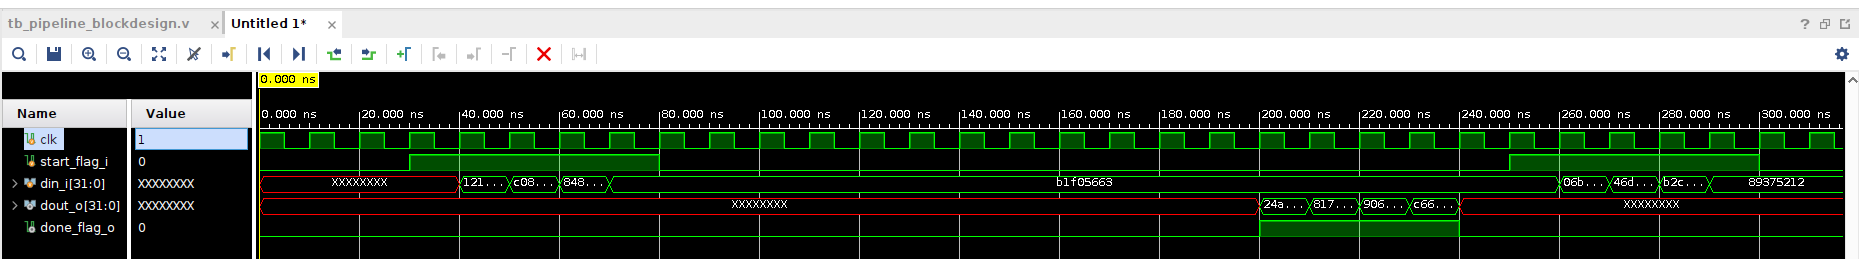
\includegraphics[width=15cm, height=2cm]{figures/simVivado.png}
  \caption{Simulación de Vivado vista con su visor integrado}
  \label{fig:simVivado}
\end{figure}

Como puede apreciarse, el comportamiento es acorde a lo esperado en el programa \textit{testbench} y en el diseño a probar: en la simulación se observa la señal de reloj \texttt{clk}, que marca el ritmo de todo el sistema. Al inicio, entre 0 ns y 40 ns, la señal de inicio \texttt{start\_flag\_i} está en cero, lo que significa que no se ha dado ninguna orden para comenzar. En ese mismo intervalo, la entrada de datos \texttt{din\_i} y la salida \texttt{dout\_o} permanecen en valores indefinidos ($\mathrm{X}$), mientras que la señal de fin \texttt{done\_flag\_o} también está en cero. Después, la entrada \texttt{din\_i} empieza a cargarse con valores concretos como \texttt{121...}, \texttt{c08...} y \texttt{648...}. El testbench está aplicando datos a la entrada para que el \textit{pipeline} comience a procesarlos. En este punto, la salida \texttt{dout\_o} sigue sin tener un valor válido. Esta latencia se debe precisamente a los ciclos necesarios para poder obtener los enteros con sus bits ya invertidos.

Más adelante, \texttt{done\_flag\_o} se pone a 1, y comienzan a aparecer cambios en la salida \texttt{dout\_o}, que muestra los valores con la inversión aplicada, como \texttt{24a...}, \texttt{817...}, \texttt{906...} y \texttt{c66...}. Este comportamiento demuestra que ya está entregando resultados y que los valores aplicados previamente en la entrada están propagándose hasta la salida. Finalmente, la salida \texttt{dout\_o} se estabiliza en el valor \texttt{89375212}, pues no se resetea ni se vuelve $\mathrm{X}$. Este momento marca la finalización del procesamiento, y se queda a la espera de la siguiente vez que se suceda el ciclo, algo que puede verse al final en la propia figura. Esto ocurrirá otras dos veces más, siendo cuatro el total, tal y como se especifica en el testbench.
\end{adjustwidth}

\subsubsection{Simulaciones en EdaPlayground}
EdaPlayground, herramienta ya detallada en \ref{st:edaplayground}, también ha sido empleada para realizar pruebas sobre el diseño. 

\vspace{0.4em} % Espacio vertical entre párrafos

\begin{adjustwidth}{1.5cm}{}
\textbf{Testbench desarrollado} \vspace{0.25cm} \\
El programa desarrollado para realizar las simulaciones en EdaPlayground es idéntico al de Vivado, presentado en \ref{lst:testbenchVivado}, salvo por la introducción de \emph{\$dumpvars(0, tb\_pipeline\_blockdesign);} al inicio de la ejecución del \textit{testbench}
\end{adjustwidth}

\vspace{0.4em} % Espacio vertical entre párrafos

\begin{adjustwidth}{1.5cm}{}
\textbf{Resultados} \vspace{0.25cm} \\
Tras aplicar dichas modificaciones, se ha realizado una simulación y descargado los resultados, para poder ver el diagrama de onda en la aplicación GTKwave, mencionada en \ref{st:gtkwave}. El resultado se presenta en la figura \ref{fig:simEdaPlayground}.

\begin{figure}[!ht]
  \centering
  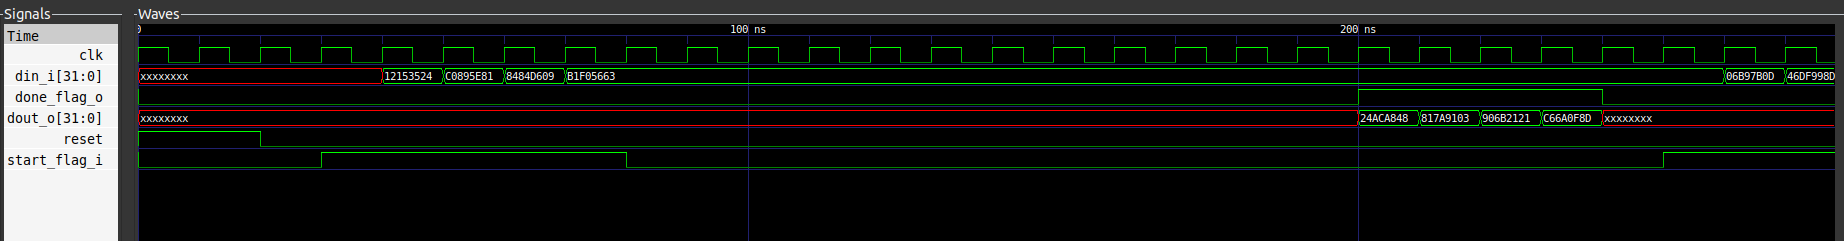
\includegraphics[width=15cm, height=2cm]{figures/simEdaPlayground.png}
  \caption{Simulación de EdaPlayground vista con GTKWave}
  \label{fig:simEdaPlayground}
\end{figure}

Como puede apreciarse, el comportamiento es equivalente al del resultado realizado con Vivado; al inicio, durante el \textit{reset}, las señales de entrada y salida están en estado indefinido ($\mathrm{X}$). Una vez que el \textit{reset} baja, se activa \texttt{start\_flag\_i} y el módulo comienza a capturar valores en \texttt{din\_i}. Tras varios ciclos de reloj de procesamiento, aparecen datos válidos en \texttt{dout\_o}, acompañados por la activación de \texttt{done\_flag\_o}, que indica que los resultados ya están listos. Finalmente, \texttt{done\_flag\_o} vuelve a cero y regresa a un estado indefinido ($\mathrm{X}$). Más adelante, tal y como se puede ver al final del diagrama, se repite de nuevo todo el ciclo de operación, algo que ocurrirá otras dos veces más hasta llegar a cuatro, pues así se definió en el \textit{testbench}.
\end{adjustwidth}

\subsection{Iteración 4 - Integración del diseño en X-HEEP}

\subsection{Iteración 5 - Ejecución del diseño en X-HEEP sobre FreeRTOS}

\subsection{Iteración 6 - Comparativa de resultados frente a versión software}
